

%% AP Physics MC Questions Archive
%%----------------------------------------


%% One Dimensional Collisions
%%----------------------------------------
\element{ap}{
\begin{question}{1d-collision-q01}
    Two objects collide perfectly elastically and are isolated from all external forces.
    Which of the following statements is necessarily true?
    \begin{choices}
        \wrongchoice{Potential energy is conserved and kinetic energy is not conserved.}
        \wrongchoice{Total linear momentum is conserved and the velocity of the objects will be of equal magnitude, but opposite direction.}
        \wrongchoice{The objects will stick together and move as one after the collision.}
      \correctchoice{The kinetic energy of the system after the collision is equal to the kinetic energy of the system before the collision.}
        \wrongchoice{The velocity of the objects will remain unchanged.}
    \end{choices}
\end{question}
}

\element{ap}{
\begin{question}{1d-collision-q02}
    %% Base your answer to the following question on the following situation.
    A proton and an anti-proton,
        each of mass \SI{1.67e-27}{\kilo\gram} are in the same general vicinity and have very small initial speeds.
    They then annihilate each other,
        producing two photons.
    What is the angle between the paths of the emerging photons?
    \begin{multicols}{3}
    \begin{choices}
        \wrongchoice{\ang{0}}
        \wrongchoice{\ang{45}}
        \wrongchoice{\ang{60}}
        \wrongchoice{\ang{90}}
      \correctchoice{\ang{180}}
    \end{choices}
    \end{multicols}
\end{question}
}

%\element{ap}{
%\begin{question}{1d-collision-q03}
%    A cart full of sand is rolling along a frictionless surface as a hole in the bottom of the cart allows sand to fall out at a constant rate.
%    \begin{center}
%    \begin{tikzpicture}
%        %% Vector
%        \draw[thick,->] (0,4) -- (3,4);
%        %% Cart
%        \node[very thick,fill=white!50!black,minimum width=4cm,minimum height=2cm,draw,anchor=south] (C) at (0,0.5) {};
%        \draw (C.north west) -- ++(90:0.5) -- ++(0:4cm) -- (C.north east);
%        %% Wheels
%        \node[draw,circle,anchor=north,minimum size=0.5cm] at (-1.75,0.5) {};
%        \node[draw,circle,anchor=north,minimum size=0.5cm] at (+1.75,0.5) {};
%        %% NOTE: TODO: Falling Sand?
%    \end{tikzpicture}
%    \end{center}
%    As the cart rolls and the sand falls out,
%        the speed of the cart will:
%    \begin{choices}
%        \wrongchoice{increase at a constant rate.}
%        \wrongchoice{increase at a variable rate.}
%        \wrongchoice{decrease at a constant rate.}
%        \wrongchoice{decrease at a variable rate.}
%      \correctchoice{remain the same.}
%    \end{choices}
%\end{question}
%}

\element{ap}{
\begin{question}{1d-collision-q04}
    Two balls collide head-on and stick together.
    One has an initial velocity $3v$ to the right and mass $m$.
    The other has an initial velocity $v$ to the left and mass $2m$.
    What is the final velocity of the system?
    \begin{multicols}{2}
    \begin{choices}
      \correctchoice{$\dfrac{v}{3}$ to the right}
        \wrongchoice{$\dfrac{v}{3}$ to the left}
        \wrongchoice{$v$ to the right}
        \wrongchoice{$v$ to the left}
        \wrongchoice{$2v$ to the right}
    \end{choices}
    \end{multicols}
\end{question}
}

\element{ap}{
\begin{question}{1d-collision-q05}
    A car with a mass of \SI{1 000}{\kilo\gram} moving with a velocity of \SI{2.0}{\meter\per\second} to the right collides with a car of mass \SI{1 500}{\kilo\gram} moving with a velocity of \SI{2.0}{\meter\per\second} to the left.
    The two cars stick together.
    Their speed after the collision is:
    \begin{multicols}{3}
    \begin{choices}
        \wrongchoice{\SI{0.0}{\meter\per\second}}
        \wrongchoice{\SI{0.2}{\meter\per\second}}
      \correctchoice{\SI{0.4}{\meter\per\second}}
        \wrongchoice{\SI{0.8}{\meter\per\second}}
        \wrongchoice{\SI{1.0}{\meter\per\second}}
    \end{choices}
    \end{multicols}
\end{question}
}

\element{ap}{
\begin{question}{1d-collision-q06}
    Two coupled railroad cars, with a total mass of \SI{5000}{\kilo\gram},
        are moving to the right with a speed of \SI{1.0}{\meter\per\second}.
    They decouple, and one of them,
        with a mass of \SI{2000}{\kilo\gram} continues moving to the right with a speed of \SI{10.0}{\meter\per\second}.
    What is the speed of the second car after they decouple?
    \begin{multicols}{3}
    \begin{choices}
        \wrongchoice{\SI{1.0}{\meter\per\second}}
        \wrongchoice{\SI{2.0}{\meter\per\second}}
      \correctchoice{\SI{5.0}{\meter\per\second}}
        \wrongchoice{\SI{9.0}{\meter\per\second}}
        \wrongchoice{\SI{10}{\meter\per\second}}
    \end{choices}
    \end{multicols}
\end{question}
}

\element{ap}{
\begin{question}{1d-collision-q07}
    Two objects having the same mass travel toward each other on a flat surface,
        each with a velocity of \SI{2.0}{\meter\per\second}.
    The objects collide head-on and are reported to rebound after the collision without deformation,
        each with a speed of \SI{1.0}{\meter\per\second}.
    Which of the following assessments of this report is most accurate?
    \begin{choices}
        \wrongchoice{The report is false because momentum is not conserved.}
        \wrongchoice{The report is false because kinetic energy is not conserved.}
      \correctchoice{The report could be true if energy was lost to the environment.}
        \wrongchoice{The report could be true if there was no friction between the objects.}
        \wrongchoice{The report could be true if the surface was inclined.}
    \end{choices}
\end{question}
}

%\element{ap}{
%\begin{question}{1d-collision-q08}
%    %% Base your answer to the following question on the following information.
%    Two balls of different masses are set at a height of \SI{3}{\meter} above the ground on a frictionless table.
%    The ball on the left is of mass $2M$ and the ball on the right has a mass of $3M$.
%    They both are released simultaneously and slide onto the part of the table \SI{2}{\meter} above the ground.
%    \begin{center}
%    \begin{tikzpicture}
%        %% NOTE: TODO: wierd graphic
%    \end{tikzpicture}
%    \end{center}
%    Consider this situation:
%    The balls collide and travel \SI{1}{\meter\per\second} to the right sticking together.
%    What is the final momentum of the system?
%    \begin{multicols}{3}
%    \begin{choices}
%        \wrongchoice{$M\,\si{\kilo\gram\meter\per\second}$}
%        \wrongchoice{$2M\,\si{\kilo\gram\meter\per\second}$}
%        \wrongchoice{$3M\,\si{\kilo\gram\meter\per\second}$}
%        \wrongchoice{$4M\,\si{\kilo\gram\meter\per\second}$}
%      \correctchoice{$5M\,\si{\kilo\gram\meter\per\second}$}
%    \end{choices}
%    \end{multicols}
%\end{question}
%}

\element{ap}{
\begin{question}{1d-collision-q09}
    A \SI{100}{\kilo\gram} cannon at rest is loaded with a \SI{10}{\kilo\gram} cannon ball.
    When fired horizontally, the cannon ball leaves the cannon with a speed of \SI{90}{\meter\per\second}.
    What is the recoil speed of the cannon?
    \begin{multicols}{3}
    \begin{choices}
        \wrongchoice{\SI{4.5}{\meter\per\second}}
      \correctchoice{\SI{9}{\meter\per\second}}
        \wrongchoice{\SI{18}{\meter\per\second}}
        \wrongchoice{\SI{90}{\meter\per\second}}
        \wrongchoice{\SI{81}{\meter\per\second}}
    \end{choices}
    \end{multicols}
\end{question}
}

\element{ap}{
\begin{question}{1d-collision-q10}
    A locomotive is traveling at \SI{50}{\meter\per\second} and it couples to another train car of the same mass at rest.
    What is the resulting velocity of the locomotive,
        train car system?
    \begin{multicols}{2}
    \begin{choices}
        \wrongchoice{\SI{50}{\meter\per\second}}
        \wrongchoice{\SI{100}{\meter\per\second}}
      \correctchoice{\SI{25}{\meter\per\second}}
        \wrongchoice{\SI{75}{\meter\per\second}}
        \wrongchoice{The system comes to a stop}
    \end{choices}
    \end{multicols}
\end{question}
}

\element{ap}{
\begin{question}{1d-collision-q11}
    A small airplane of mass \SI{5000}{\kilo\gram} holding a package of \SI{500}{\kilo\gram} is traveling at \SI{60}{\meter\per\second}.
    The airplane releases this package.
    What is the speed of the airplane after the release?
    \begin{multicols}{3}
    \begin{choices}
        \wrongchoice{\SI{33}{\meter\per\second}}
      \correctchoice{\SI{60}{\meter\per\second}}
        \wrongchoice{\SI{66}{\meter\per\second}}
        \wrongchoice{\SI{63}{\meter\per\second}}
        \wrongchoice{\SI{54}{\meter\per\second}}
    \end{choices}
    \end{multicols}
\end{question}
}

\element{ap}{
\begin{question}{1d-collision-q12}
    %Base your answers to questions 12 through 14 on the following scenario:
    A \SI{1}{\kilo\gram} ball of clay is moving at \SI{2}{\meter\per\second} when it strikes an object at rest with a mass of \SI{5}{\kilo\gram}.
    The objects move together as one after the impact.
    %% start question
    The kinetic energy of the two objects before the impact is:
    \begin{multicols}{3}
    \begin{choices}
        \wrongchoice{\SI{1}{\joule}}
      \correctchoice{\SI{2}{\joule}}
        \wrongchoice{\SI{8}{\joule}}
        \wrongchoice{\SI{12}{\joule}}
        \wrongchoice{\SI{24}{\joule}}
    \end{choices}
    \end{multicols}
\end{question}
}

\element{ap}{
\begin{question}{1d-collision-q13}
    %Base your answers to questions 12 through 14 on the following scenario:
    A \SI{1}{\kilo\gram} ball of clay is moving at \SI{2}{\meter\per\second} when it strikes an object at rest with a mass of \SI{5}{\kilo\gram}.
    The objects move together as one after the impact.
    %% start question
    The velocity of the two objects after the collision is most nearly:
    \begin{multicols}{3}
    \begin{choices}
        \wrongchoice{\SI{0.1}{\meter\per\second}}
        \wrongchoice{\SI{0.2}{\meter\per\second}}
      \correctchoice{\SI{0.3}{\meter\per\second}}
        \wrongchoice{\SI{0.4}{\meter\per\second}}
        \wrongchoice{\SI{0.5}{\meter\per\second}}
    \end{choices}
    \end{multicols}
\end{question}
}

\element{ap}{
\begin{question}{1d-collision-q14}
    The ratio of the initial kinetic energy to the kinetic energy after the collision of the two balls is most nearly:
    \begin{multicols}{3}
    \begin{choices}
        \wrongchoice{$1:1$}
        \wrongchoice{$1:2$}
        \wrongchoice{$1:3$}
        \wrongchoice{$2:1$}
      \correctchoice{$6:1$}
    \end{choices}
    \end{multicols}
\end{question}
}

\element{ap}{
\begin{questionmult}{1d-collision-q15}
    Two isolated objects collide in an inelastic collision.
    Which of the following statements is/are correct?
    \begin{choices}
      \correctchoice{Total energy is conserved}
        \wrongchoice{Kinetic energy is conserved}
      \correctchoice{Linear momentum is conserved}
    \end{choices}
\end{questionmult}
}

\element{ap}{
\begin{question}{1d-collision-q16}
    A railroad car of mass $m$ is moving due west with a velocity $v$.
    A locomotive of mass $M$ drives due east on the same track and couples together with the car.
    What velocity must the locomotive be traveling so that the locomotive and car system will come to rest after the collision?
    \begin{multicols}{2}
    \begin{choices}
        \wrongchoice{$-\dfrac{Mv}{M+m}$}
        \wrongchoice{$-\dfrac{mv}{M+m}$}
        \wrongchoice{$-\dfrac{Mv}{m}$}
        \wrongchoice{$-\dfrac{mv}{M}$}
      \correctchoice{$-\dfrac{\left(M+m\right)v}{M}$}
    \end{choices}
    \end{multicols}
\end{question}
}

\element{ap}{
\begin{question}{1d-collision-q17}
    %% Base your answers to questions 17 and 18 on the following situation.
    A railroad car of mass $m$ is moving at a velocity $v$ when it collides with a second railroad car,
        at rest, of mass $2m$ at rest.
    The two cars lock together instantaneously and move along the track.
    %% Start question
    What is the speed of the cars immediately after the collision?
    \begin{multicols}{3}
    \begin{choices}
        \wrongchoice{$\dfrac{v}{2}$}
      \correctchoice{$\dfrac{v}{3}$}
        \wrongchoice{$v$}
        \wrongchoice{$2v$}
        \wrongchoice{$3v$}
    \end{choices}
    \end{multicols}
\end{question}
}

\element{ap}{
\begin{question}{1d-collision-q18}
    %% Base your answers to questions 17 and 18 on the following situation.
    A railroad car of mass $m$ is moving at a velocity $v$ when it collides with a second railroad car,
        at rest, of mass $2m$ at rest.
    The two cars lock together instantaneously and move along the track.
    %% Start question
    What is the change in kinetic energy of the cars as a result of the collision?
    \begin{multicols}{3}
    \begin{choices}
        \wrongchoice{$\dfrac{mv^2}{9}$}
        \wrongchoice{$\dfrac{mv^2}{4}$}
      \correctchoice{$\dfrac{mv^2}{3}$}
        \wrongchoice{$\dfrac{mv^2}{2}$}
        \wrongchoice{$mv^2$}
    \end{choices}
    \end{multicols}
\end{question}
}

\element{ap}{
\begin{question}{1d-collision-q19}
    In the below diagram,
        a \SI{1000}{\kilo\gram} spacecraft is traveling at a velocity of \SI{200}{\meter\per\second} in the $+x$ direction when it ejects a \SI{200}{\kilo\gram} payload at \SI{10}{\meter\per\second} in the $+y$ direction.
    \begin{center}
    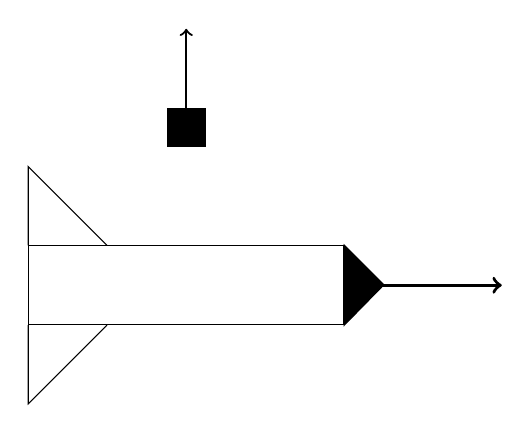
\begin{tikzpicture}
        %% Rocket
        \node[minimum width=4cm,minimum height=1cm,draw] (R) at (0,0) {};
        \draw[fill] (R.north east) -- ++(-45:0.71) -- (R.south east) --cycle;
        \draw (R.north west) -- ++(90:1cm) -- ++(-45:1.414);
        \draw (R.south west) -- ++(270:1cm) -- ++(45:1.414);
        %% Payload
        \node[minimum size=0.5cm,fill] (P) at (0,2) {};
        %% Vectors
        \draw[thick,->] (P.north) -- ++(90:1cm);
        \draw[very thick,->] (R.east) -- ++(0:2cm);
    \end{tikzpicture}
    \end{center}
    The velocity of the spacecraft in the $x$ direction is now:
    \begin{multicols}{3}
    \begin{choices}
      \correctchoice{\SI{200}{\meter\per\second}}
        \wrongchoice{\SI{250}{\meter\per\second}}
        \wrongchoice{\SI{212}{\meter\per\second}}
        \wrongchoice{\SI{238}{\meter\per\second}}
        \wrongchoice{\SI{240}{\meter\per\second}}
    \end{choices}
    \end{multicols}
\end{question}
}

\element{ap}{
\begin{question}{1d-collision-q20}
    Which of the following is conserved in an elastic collision but not in an inelastic collision?
    \begin{choices}
        \wrongchoice{linear momentum}
        \wrongchoice{angular momentum}
      \correctchoice{kinetic energy}
        \wrongchoice{total energy}
        \wrongchoice{mass}
    \end{choices}
\end{question}
}

\element{ap}{
\begin{question}{1d-collision-q21}
    Two people, each of mass \SI{50}{\kilo\gram},
    are sliding together at a constant velocity of \SI{4}{\meter\per\second} on frictionless ice.
    At a time $t=\SI{0}{\second}$,
        they push apart such that one of them remains at rest.
    How far apart are they after another \SI{5}{\second} has passed?
    \begin{multicols}{3}
    \begin{choices}
        \wrongchoice{\SI{0}{\meter}}
        \wrongchoice{\SI{10}{\meter}}
        \wrongchoice{\SI{20}{\meter}}
        \wrongchoice{\SI{30}{\meter}}
      \correctchoice{\SI{40}{\meter}}
    \end{choices}
    \end{multicols}
\end{question}
}

\element{ap}{
\begin{question}{1d-collision-q22}
    Compared to the final speed of the objects involved in an elastic collision and the energy lost in an elastic collision,
        an inelastic collision:
    \begin{choices}
      \correctchoice{dissipates more energy and causes lower final speeds}
        \wrongchoice{dissipates the same energy and causes lower final speeds}
        \wrongchoice{dissipates less energy and causes the same final speeds}
        \wrongchoice{dissipates more energy and causes higher final speeds}
        \wrongchoice{dissipates the same energy and causes higher final speeds}
    \end{choices}
\end{question}
}


\endinput


